\subsection{Subjects} \label{repo_analysis_subjects}

Only English subjects and those that don't have the language defined are considered here. We include subjects of unknown language because this is how edoc and refubium store the \acrshort{ddc} terms. 81 \% of all subjects occur only once, meaning they are only used by one publication. As shown in figure \ref{fig:subject_pie}, only 5 \% of the subjects are used by more than 3 publications.

Each document contains on average 3.37 subjects, with 11,091 documents (38 \%) having no subjects. The full distribution of documents over the number of subjects is plotted in figure \ref{fig:subject_bar}. The document with the most number of subjects contains 186 subjects. This document, as well as the next nine documents with the most number of subjects, all belong to edoc. In total, there are 85,564 unique subjects among all three repositories. Here, unique means that the tuple formed by the name and the subject type are unique. A subject can be of type \textit{ddc}, \textit{dnb} (German bibliography system\footnote{\url{https://docplayer.org/32389589-Sachgruppen-der-deutschen-nationalbibliografie-bis-2003.html}}), \textit{rvk} (Regensburg Network Classification Scheme), \textit{classification}, \textit{other} or \textit{unknown}.

\begin{figure}
  \begin{subfigure}[t]{0.55\textwidth}
    \centering
    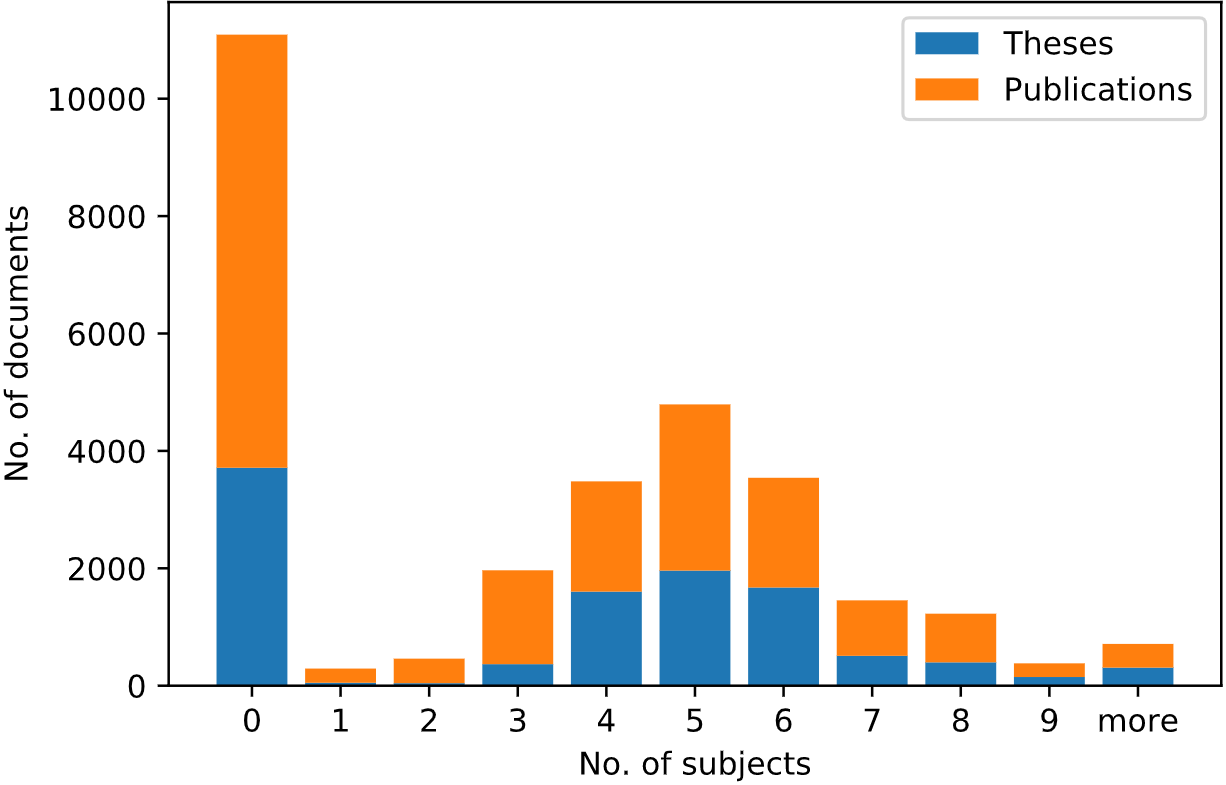
\includegraphics[width=\textwidth]{figures/repository_analysis/subjects_per_document.png}
    \caption{No. of publications for each number of subjects}
    \label{fig:subject_bar}
  \end{subfigure}
  \hfill
  \begin{subfigure}[t]{0.35\textwidth}
    \centering
    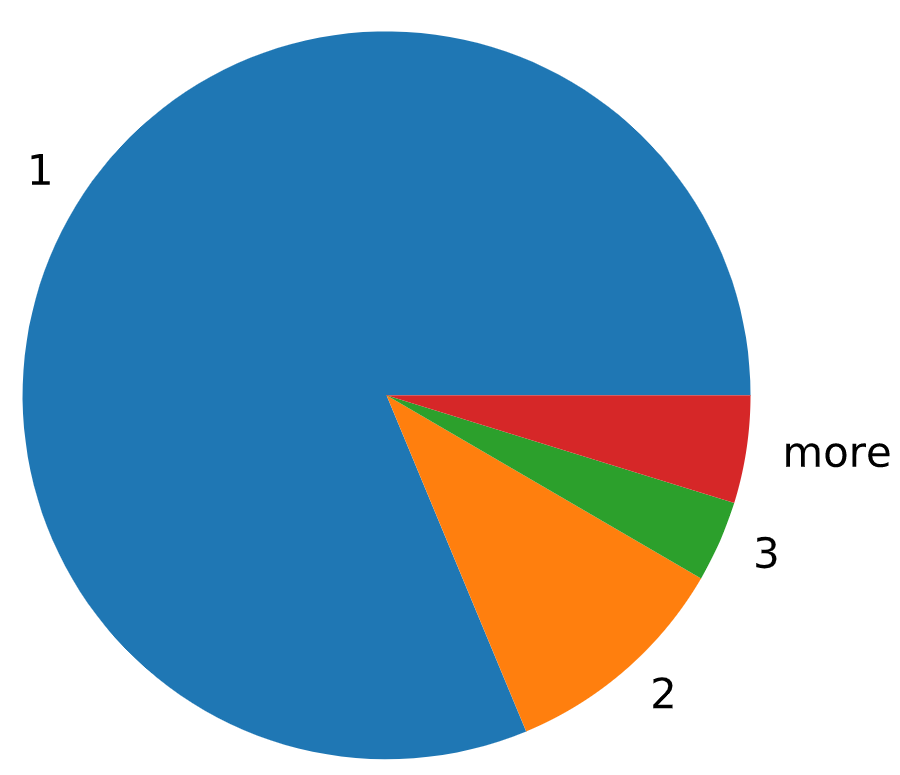
\includegraphics[width=\textwidth]{figures/repository_analysis/subject_occurrence.png}
    \caption{Subject occurrence.}
    \label{fig:subject_pie}
  \end{subfigure}
  \caption{Charts analyzing subjects of the relevant documents.}
\end{figure}

\subsubsection{DDC subjects} \label{subjects_ddc}

Many of the popular subjects belong to the \acrshort{ddc}, except for some subjects of edoc which follow the numbering system of a German bibliography system mentioned above. The \textit{ddc} subjects are reduced to the first number they contain. This is necessary because refubium stores the \acrshort{ddc} terms in a different format than edoc and depositonce. After modifying the terms, there are 390 distinct \acrshort{ddc} terms in the three repositories. The most popular subject is \textit{610 Medicine and health}, from refubium. \textit{530 Physics} is the second most popular subject, and it appears in all three repositories.  

302 of the 390 \acrshort{ddc} terms are sections, i.e. the numbers don't end in zero. Examples of sections are \textit{532 Fluid mechanics} and \textit{336 Public finance}. The sections present in the repositories are assigned to 20 documents on average. 81 of the remaining 88 \acrshort{ddc} terms are classes (numbers that end with two zeros, e.g. \textit{500 Science}) and divisions (numbers that end in zero, e.g. \textit{530 Physics}). They are assigned to over 200 documents on average. The other 7 \acrshort{ddc} terms do not include any number and must be introduced manually.

As illustrated in figure \ref{fig:ddc_distribution}, the most popular class overall is \textit{500 Science}, which is also the most popular class in refubium and depositonce. \textit{300 Social Sciences} is the most popular in edoc and third overall, slightly less popular than \textit{600 Technology}. These three classes cover 83 \% of all the relevant documents.

\begin{figure}
    \centering
    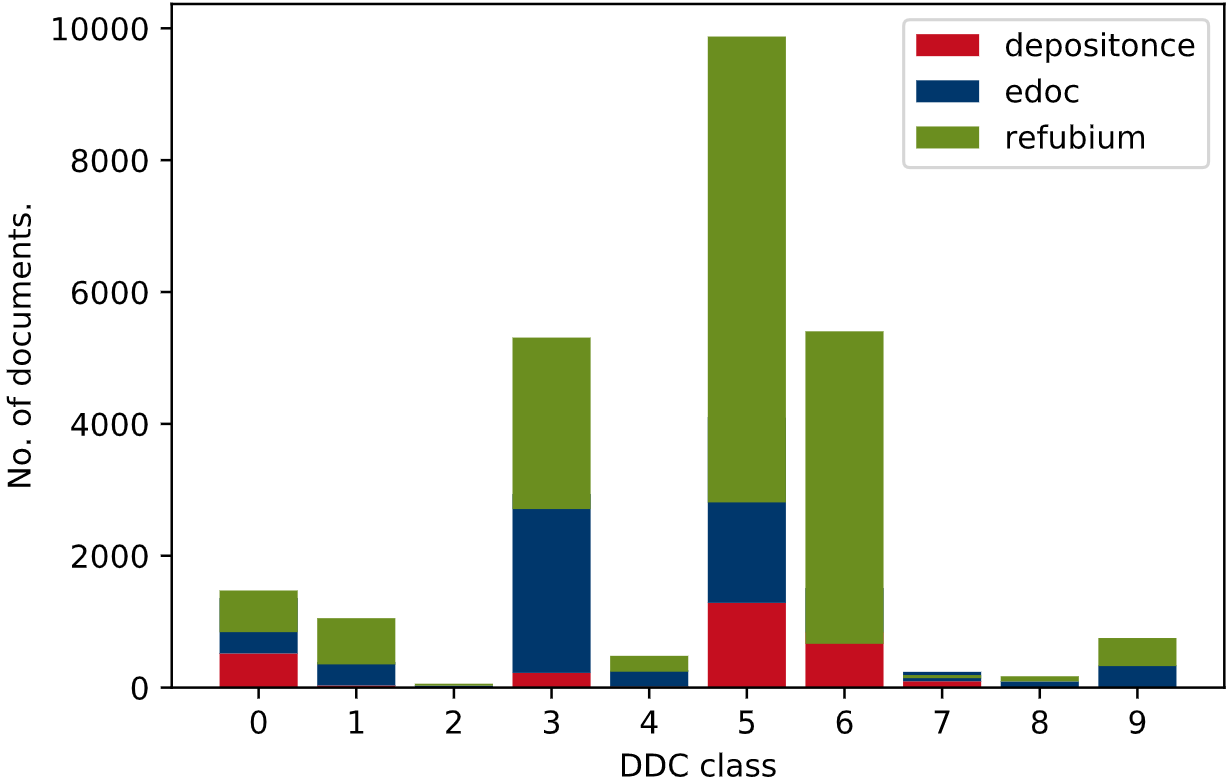
\includegraphics[width=.8\textwidth]{figures/repository_analysis/ddc_distribution.PNG}
    \caption{Distribution of the documents among the ten \acrshort{ddc} classes.}
    \label{fig:ddc_distribution}
\end{figure}

\subsubsection{Duplicate subjects} \label{subjects_duplicates}

When uploading a document to a repository, users can input subjects as free text, without any constraints. This allows for equivalent subjects to be present in different form, e.g. in lower or upper case and singular or plural. To identify potential duplicates, we have applied a pre-processing procedure outlined in KEA++'s paper \cite{medelyan2008domain}:

\begin{enumerate}
    \item Lower-case all characters.
    \item Tokenize the subjects.
    \item Filter out stop words.
    \item Stem the remaining words.
    \item Order the stems alphabetically.
\end{enumerate}

This procedure identified 13,412 duplicate subjects. Some of these only appear once in the repositories. Merging them results in 7 \% fewer subjects that occur only once.